\documentclass[a4paper]{article}

\usepackage[english]{babel}
\usepackage[utf8]{inputenc}
\usepackage{amsmath}
\usepackage{graphicx}
\usepackage[colorinlistoftodos]{todonotes}
\usepackage{float}
\usepackage{subfigure}
\usepackage{subfloat}

\title{CS294 Deep RL Assignment 5: Exploration Strategies}

\author{Mohamed Khodeir}

\date{\today}

\begin{document}
\maketitle


\section*{Problem 1}
\begin{figure}[H]
\centering
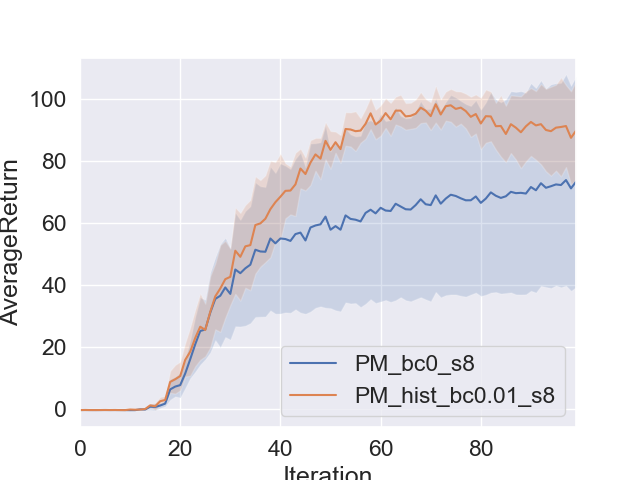
\includegraphics[width=1\textwidth]{p1.png}
\caption{Comparing an agent with histogrambased exploration and an agent with no exploration.}
\end{figure}

\pagebreak

\section*{Problem 2}
\begin{figure}[H]
\centering
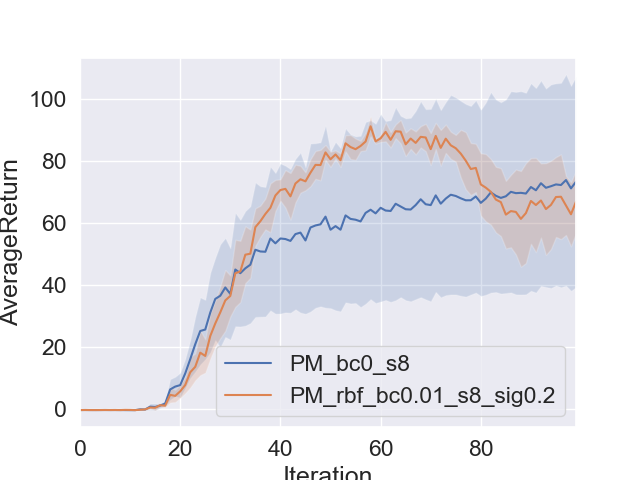
\includegraphics[width=1\textwidth]{p2.png}
\caption{Comparing an agent with KDEbased exploration and an agent with no exploration.}
\end{figure}

\pagebreak

\section*{Problem 3}
\begin{figure}[H]
\centering
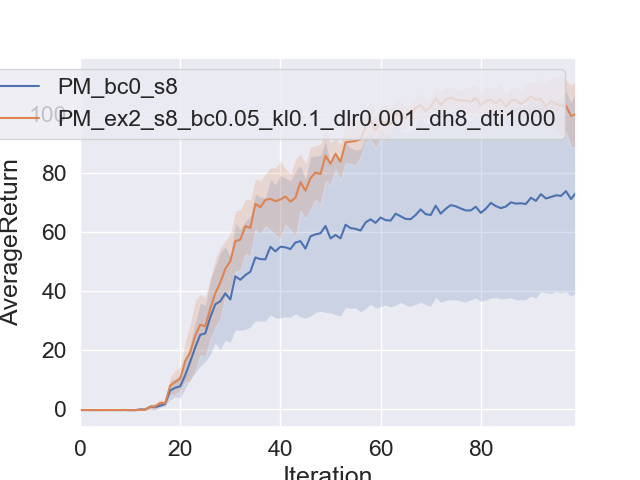
\includegraphics[width=1\textwidth]{p3.png}
\caption{Comparing an agent with EX2-based exploration and an agent with no exploration.}
\end{figure}

\pagebreak

\section*{Problem 4}
\begin{figure}[H]
\centering
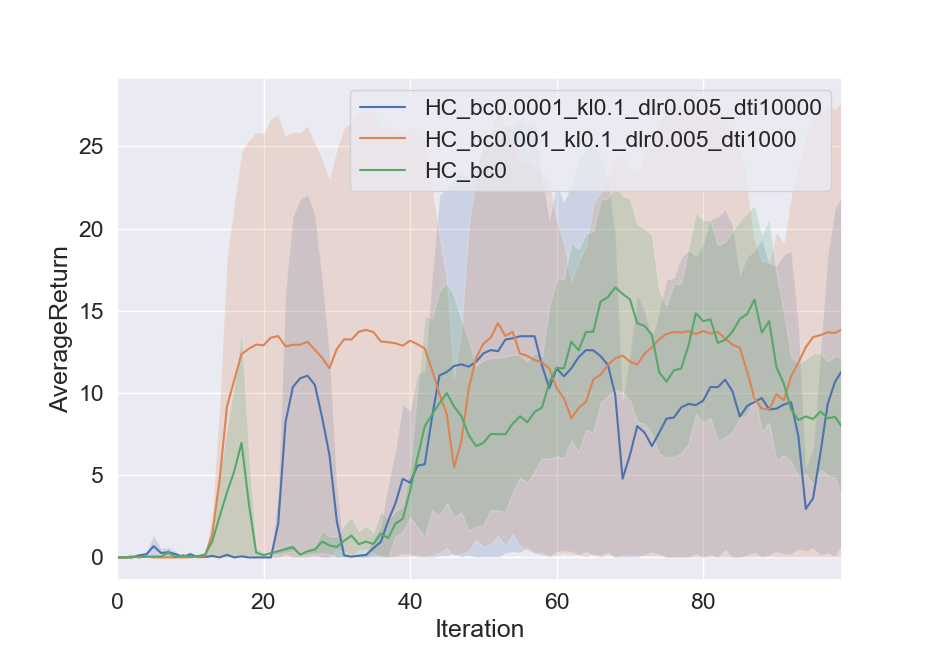
\includegraphics[width=1\textwidth]{p4.png}
\caption{Comparing the agents with EX2-based exploration and an agent with no exploration.}
\end{figure}

In this experiment, we varied the bonus coefficient as well as the number of iterations on which the descriminator was trained. (1) With regard to the shape of the curves, one obvious thing to note is that the curve corresponding to the higher bonus coefficient seems to display significantly faster improvements in AverageReturn. However, both display faster improvement than the run without an exploration bonus. This could be attributed to faster exploration early on (as higher weight is given to novel states). This also explains to some extent, the higher variance (evident on the error bands) as more exploration is done vs exploitation of known good states. The difference in variance between the two ex2 runs, might also be explained to some extent by the difference in the number of iterations for which the discrimnator was trained. Intuitively, perhaps the discrimnator, having not been trained to convergence, displays higher variance in its state novelty estimation. (2) There is not a significant difference between the peak performance of the runs. Surprisingly, the run with a higher bonus coefficient seems to be more stable. I would have expected the opposite as more weight is given to exploration of unknown states should cause more fluctuations in average return.

\end{document}
